%!TEX root = ../dissertation.tex

\chapter{INTRODUCTION}
%\begin{spacing}{1.9}

\section{General introduction and organizaion of the dissertation}
In many instances, it is useful to view data as a collection of curves. The study of human growth is a common example used to motivate this view, where data arising from the study can be viewed as collection of individual growth curves.  The second derivative of the growth curves are used to study growth acceleration and identify common growth spurts. In studies like this, where the questions motivating the analysis relate to properties of curves, it makes sense to view the fundamental datum as a curve and refer to the collection of curves as \emph{functional data}.  \cite{ferraty2006nonparametric} characterize this by defining a functional random variable as one which takes values in an infinite dimensional space. 

The publication of the book \emph{Functional Data Analysis}---the seminal work by \cite{FDA}---inspired substantial interest in developing statistical models for functional data.  Though their book describes the extension of linear models to the functional setting, it stops short of allowing for complex dependence structures by assuming independence between observed curves. For curves observed in space, this assumption is often violated. Examples of functional data which have a spatial index are becoming more common in scientific studies: data collected by weather stations, oceanology measurements taken by seals equipped with sensor devices, peak electron density measurements collected by ionosonde stations in the northern hemisphere, and satellite measurements of environmental variables. Therefore,  research on functional models for spatial data is a very important and actual topic.

 In environmental data,  the correlations exhibited between observations in space may be of scientific interest and often the primary goal of the analysis is prediction of a environmental variable at an unobserved location.  In this setting, geostatistical models are often used. The extension of geostatistical models for functional data were first considered by \cite{Goulard:1993}, who proposed two possible approaches: one approach involves cokriging by reducing the functional response to a multivariate response, while the other approach untilizes a functional version of the variogram.  The functional variogram approach has been further developed by \cite{Giraldo:2010jx} and \cite{Nerini:2010ba}.

%Examples of spatially indexed functional data have also been considered for functional data with a multilevel structure, often arising in the case of designed experiments. In these cases, a mixed model framework is typically used and much work has been done extending mixed model methodology to accommodate functional observations (\cite{Li:2007dn}, \cite{Morris:2006wq},\cite{Di:2009dz}, \cite{Baladandayuthapani2008},\cite{Staicu:2010ez}, \cite{Scheipl:2012tm}). 

When data are random curves rather than scalars or vectors, it is necessary to have a convenient way to represent the curves.  A standard approach is to express the curves in terms of a known basis set (e.g. b-spline, wavelets, Fourier). An alternative, and what we believe to be a more attractive choice for spatial functional data, is an empirical basis consisting of functional principal components (FPC). FPCs are able to reduce infinite dimensional functional data to a finite dimension in an optimal way. When curves are represented by a linear combination of basis functions, the variation among curves can be investigated through the variation among the coefficients of the basis functions. Thus, spatial similarity between curves can be modeled through the correlation structure associated with the basis function coefficients viewed as multivariate random fields. Using a finite basis representation of the curves, each curve is identified by its vector of coefficients, allowing the use of multivariate methods; moreover, it is well known that principal components achieve maximum efficiency in terms of representing variation in the data for a fixed dimension. 

To clarify what is meant by functional principal components, we present here a brief review of the relevant mathematical results.
A process $X(t)$, defined on a closed interval $\T  \subset \Real$,  with finite covariance possesses a sequence of orthonormal eigenfunctions $\{\psi_m(t)\}_{m=1,2,\ldots}$, which form a complete basis for the space, with associated nonnegative and nondecreasing eigenvalues $\{\lambda_m \}_{m=1,2,\ldots}$. By the Karhunen-Loeve expansion, the process $X(t)$ admits the representation
\begin{equation*}
X(t) =  \sum_{m=1}^{\infty}\alpha_m \psi_m(t), \mbox{ where  } \alpha_m = \int_{\T} X(t) \psi_m(t)dt.
\end{equation*}

The random variables $\{\alpha_m \}_{m=1,2,\ldots}$ are the functional principal component scores of $X(t)$, which are uncorrelated and satisfy $E(\alpha_m)=0$ and var($\alpha_m$) = $\lambda_m$, $\sum_m \lambda_m < \infty$.\\
Remarks:
\begin{enumerate}
	\item The eigenfunctions are orthonormal in the space $L^2[\T]$ and the FPC scores are uncorrelated random variables.
	\item The eigenfunctions efficiently capture the dominant modes of variation in the observed curves.
	\item The eigenvalues often decrease rapidly and thus the infinite dimensional process $X(t)$ can be well approximated by a small number of FPCs.
\end{enumerate}

This framework is often adopted (e.g., \cite{Yao:2005cv,Di:2009dz,Gromenko:2012ij}); however, 
this approach introduces the non-trivial problem of estimating the principal component functions from observed data. Estimation of principal component functions can be accomplished by estimating the covariance function through bivariate smoothing and then computing the eigenfunctions of the estimated covariance surface (some alternative methods are described in \cite{FDA} Ch. 8 and Ch. 9). Because of this, much effort has been devoted to methods for nonparametric covariance estimation and eigenfunction estimation ( \cite{Yao:2005cv}, \cite{Li:2007dn}, \cite{Cai:2010vr}).  Of the literature on nonparametric covariance function estimation, \cite{Cai:2010vr} provides the most general framework by assuming curves belong to a reproducing kernel Hilbert space (RKHS) and utilizing theoretical results developed for spline smoothing methods. This framework allows for closed form estimation of the eigenfunctions and their derivatives, so one does not need to discretize the covariance function and approximate eigenfunctions with eigenvectors.  This is particularly useful because we use eigenfunctions as a basis set for further model building and not just as an exploratory tool. 

In this dissertation we work in a reproducing kernel Hilbert space framework, representing curves with a principal component function basis, and model spatial dependence between curves through FPC scores.  
\begin{itemize}
\item In Chapter \ref{ch:covariance estimation} we describe an estimator for principal component functions. We have developed an R implementation of this method. In our implementation one can easily produce list object containing the estimated principal component functions. We have also developed an empirical basis specification  within the fda package framework, so that the estimated principal component functions can be used as a basis object.  %Ramsay and Silverman have stated that a future fda release will contain support for empirical bases, but I do not believe this has been implemented yet. 

\item In Chapter \ref{ch:functional kriging} we describe how this framework can be used for ordinary kriging prediction for functional data. We also describe our current work on improving the nonparametric covariance estimator by incorporating spatial dependence in the estimation of the covariance function. 

\item  In Chapter \ref{phenology} we develop a functional data analysis approach to classify vegetation patterns over a subregion of India. The data set we work with is the Merris Terestrial Cholorophyll Index (MTCI) collected by satellite at a time interval of 8 days at a 4.6~km spatial resolution over a 230~km by 230~area of southern India. Observed MCTI values over a year characterize vegetation life-cycle and are closely associated with vegetation type. The connection between vegetation land cover and phenological signal motivates a functional data analysis approach to classification of land cover based on the observed phenological signal. We employ the methodology in Chapter \ref{ch:covariance estimator} and Chapter \ref{ch:functional kriging} to estimate functinal observation in term of FPC expansions, and utilize this representation to perform classification on the resulting low-dimensional coefficent vectors. 

\item In order to make this document more self contained, Section \ref{ch:theoretical background} contains some of the relavent theoretical background related to RKHS and its role in statistics. 
\end{itemize}


\section{Theoretical background on smoothing splines and reproducing kernel Hilbert space}
 \label{ch:theoretical background}


\subsection{Historical note on the use of reproducing kernel Hilbert spaces in statistics}

This section contains some historical context to understand the motivation for the mathematical framework of reproducing kernel Hilber space and their use in statistics. In the following I would like to describe a little bit about how these special Hilbert spaces became mainstream in statistics and mention some of the key players. 
%\begin{figure}[h] %  figure placement: here, top, bottom, or page
%   \centering
%      \begin{subfigure}[b]{0.40\textwidth}
%                \centering
%                
\includegraphics[width=.5\textwidth]{Images-general-introduction/parzen.pdf}
%                %\caption{Emanuel Parzen}
%                \label{}
%        \end{subfigure}%
%        \begin{subfigure}[b]{0.40\textwidth}
%                \centering
%                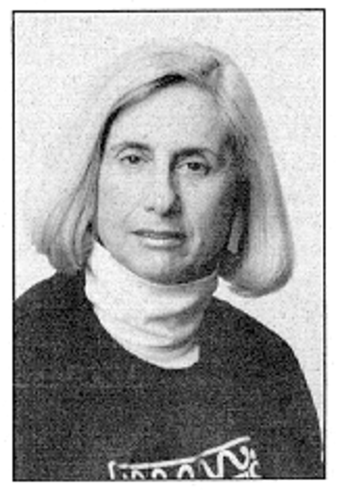
\includegraphics[width=.5\textwidth]{Images-general-introduction/wahba.pdf}
%                %\caption{Grace Wahba}
%                \label{}
%        \end{subfigure}
%   \caption{Emanuel Parzen and Grace Wahba}
%   \label{fig:example}
%\end{figure}


The origin of reproducing kernel Hilbert space methods in statistics is due to Emanuel Parzen. In an interview in a 2002 issue of Statistical Science, Parzen describes how he was introduced to the topic. He states that when he was a graduate student at Berkely, students did not take the usual Ph.D qualifying exam; instead, each student was tasked with giving a lecture to their committee on a specific topic --- Parzen's topic: reproducing kernels. When he began studying the topic, he only found one source in the literature and it was in French. The paper he found was work by Aronszajn, who had developed the abstract theory of reproducing kernels to generalize kernel methods popular in applied mathematics. 

The use of Hilbert space methods to model continuous-parameter time series appears to be the Parzen's initial application of reproducing kernels in statistics. Though Parzen was working on time series analysis, it seems that the reproducing kernel framework is used more widely in the smoothing spline methods as a regularization approach for nonparametric curve estimation due to the fact that minimization problems over a RKHS have a unique solution with a finite dimensional representation (the so-caledl representer theorem). It was Parzen's graduate student Grace Wahba who championed regularization via RKHS in her book, \emph{Spline Models for Observational Data} (\cite{Wahba:1990}). Most of the current work using a RKHS framework for nonparametric estimation cite WahbaÕs work, and it is telling that a lot of the current researchers on smoothing spline methods are themselves former students of Grace Wahba (e.g. Chong Gu, Yuedong Wang, Ming Yuan, Doug Nychka). In the introduction to her book, Grace Wahba offers some encouragement, which I have included below in quotations. I took this advice to heart when I first embarked on this topic --- I have to say that she has been true to her word. 
\begin{quote}
``I would like to assure the reader that the effort to master the basic properties of reproducing kernel Hilbert spaces, will be worth the effort.''\\
-Grace Wahba
\end{quote}

\subsection{ Going beyond ordinary least squares: Penalized least squares and the cubic smoothing spline} 


\subsubsection{Least Squares Estimation}
Consider the regression problem where observations $(x_i, y_i), i=1,\dots,n,$ are modeled as $y_i = f(x_i) + \epsilon_i, \epsilon_i \sim N(0,\sigma^2).$ This model assumes that we observe an underlying signal, $f$, corrupted by noise. The desire is to recover $f$ from the observations $(x_i, y_i), i=1,\dots,n$. The noise terms $\{\epsilon_i\}$ are random variables and exact recovery of $f$ is not possible, thus our goal becomes to find a good approximation to $f$. The least squares estimator of $f$ is given by the minimizer $\hat{f}$ of the sum of the squared deviations over all functions $f \in \mathcal{A}$ 
\begin{equation*}
\hat{f} = \hspace{.07in} \stackrel[f \in \mathcal{A}]{}{\mbox{argmin}} \frac{1}{n}\sum_{i=1}^{n}(y_i - f(x_i))^2.
\label{eq:LS}
\end{equation*}

If the underlying signal $f$ does not lie in $\A$, then the estimator is guaranteed to be biased. In order to avoid misspecification of $\A$, a wide class of functions should be considered.  As a concrete example, in simple linear regression we have $\A = \{f: f(x_i) = \beta_0 + \beta_1x_i ; i=1,\dots,n \}$. In this setting, $\A$ is defined as the two dimensional subspace of $\Real^n$ spanned by a column of 1s and the column vector $(x_1,\dots, x_n)'$. The matrix consisting of these columns constitutes the \textit{model matrix.} Any function $f \in \A$ can be identified uniquely by the parameters $\beta_0$ and $\beta_1$ in its representation as a linear combination of the columns of the model matrix. Thus, the solution to the least squares minimization problem has the representation $\wh{f} = X\wh{\bbeta}$ satisfying 
\begin{equation*}
\widehat{\bbeta} =  \hspace{.07in}  \stackrel[\bbeta \in \Real^2]{}{\mbox{argmin}} (\textbf{Y} - \textbf{X}\bbeta)'(\textbf{Y} - \textbf{X}\bbeta)
\label{eq:LS2}
\end{equation*}
where $\textbf{Y}=(y_1,\dots, y_n)'$, and $\textbf{X}$ is the model matrix. Finding $\widehat{\bbeta}$ requires simple matrix calculus manipulations. 

\subsubsection{Penalized Least Squares} \label{PLS}
  The purpose of presenting the simple linear regression problem in the previous section was to emphasize how the choice of a parametric model can be framed as a choice of the structure of the function space $\A$. The simple linear regression model is equivalent to specifying $\A$ to be a known 2-dimensional subspace of $\Real^n$ -- the column space of $\textbf{X}$. In practice, many relationships of interest are approximately linear making this model suitable in such cases. However, in most applications it is not the \textit{truth} of the model we believe in, but its adequacy as a mathematical representation of the underlying relationship. When a parametric model is adequate the parameters often give us insight into the structure of the relationship and scientific questions of interest can often be stated in using contrasts of the parameters. However, there is usually very little known about the functional form of $f$, and hence there is very little justification for restricting the estimator to belong to a particular class of parametric functions. 
 
Therefore, it seems desirable to consider a larger class of functions. To decide on how large this class should be, we remark that any reasonably large class of functions will contain functions that interpolate the data. Since we believe the observational process is corrupted by noise, we do not wish to model the idiosyncrasies of the data; that is,  we believe the estimator $\hat{f}$ must be smoother than an interpolating function. Penalized least squares is one method where this problem is addressed by including a term that penalizes the roughness of the function. The penalized least squares estimator of $f$ is formulated to balance two competing functionals 
\begin{equation}
\widehat{f}_{\lambda} = \hspace{.07in}\stackrel[f \in \A]{}{\mbox{argmin}} \left\{ \frac{1}{n}\sum_{i=1}^{n}(y_i - f(x_i))^2 + \lambda\int_{\X}(f''(x))^2dx \right\},
\label{eq:PLS}
\end{equation}
where the smoothing parameter $\lambda$ governs the trade-off between fitting the data and smoothness of the function. In \eqref{eq:PLS} the smoothness of the function is measured by the integral of its squared second derivative, thus implicitly assuming the second derivative exists and that it is square integrable. A natural functional space to consider is the space $\A = \{f: f, f' \mbox{are absolutely continuous and } \int_0^1f''(x)^2dx <\infty\}$. It is important to note that linear functions are not penalized in \eqref{eq:PLS} and as $\lambda \rightarrow \infty$ the estimator $\wh{f_{\lambda}}$ converges to the least squares estimator. Two important questions to consider are: 
\begin{enumerate}
	\item Is there a solution to the minimization problem in \eqref{eq:PLS}?
	\item Is the solution unique?
\end{enumerate}
The answer is affirmative to both questions; furthermore, the solution is a piecewise cubic polynomial.  To better understand how to solve minimization problems like \eqref{eq:PLS} we consider the Hilbert space structure of $\A$, and show how the existence of a reproducing kernel is key. 
 

%============================================================================================================================
\subsection{Reproducing kernel Hilbert spaces (RKHS)}
%============================================================================================================================

%=======================================================================================================
\subsubsection{Notation and basic definitions}


In this section we will cover a brief introduction to reproducing kernel Hilbert spaces. Two excellent introductions to this material are given in \cite{Heckman:1997vp} and \cite{Storlie:2011tz}, while more rigorous presentations are given by \cite{Wahba:1990} and \cite{Aronszajn:1950tq}. 
Notice that in \eqref{eq:PLS} the sum of squares term involves evaluation of $f$. A reproducing kernel Hilbert space is a Hilbert space where function evaluation is a continuous linear operator. That is a Hilbert space $\H$ on a domain $\T$ is a reproducing kernel Hilbert space if $L_t(f) = f(t)$ is continuous in $\H$, $\forall t \in \T$. The domain $\T$ often represents a continuous time domain and will typically be the close interval $[0,1]$. It is well known that continuity of a linear functional is equivalent to boundedness of the functional, where boundedness means that there exists an $M_t$ such that 
\begin{equation*}
	|L_t(f)|=|f(t)|\leq M_t\norm{f}_{\H}, \mbox{ for all $f$ in the RKHS}.
\label{eq:}
\end{equation*}
The Riesz representation theorem states that any continuous linear operator on $\H$ has a representation in terms of the inner product on $\H$
\begin{equation}
	L_t(f) = \inner{R_t(\cdot)}{f(\cdot)} = f(t), \forall f\in \mathcal{H},
\label{eq:Riesz}
\end{equation}
where $R_t$ is a function in $\H$. If we denote $R_t(s)$ by $R(s,t)$, then the reproducing property in \eqref{eq:Riesz} implies that $\inner{R_s(\cdot)}{ R_t(\cdot)} = R(s,t)$. Note the $R(s,t)$ is a symmetric bivariate function defined on $\T\times\T$. %We will denote by $\H$$_R$ a RKHS with reproducing kernel R, and its inner product by $\langle\cdot,\cdot>_R$. 

At this point, we note that this reproducing property may appear to be similar to the use of the Dirac delta function $\delta$, where $f(x)=\int\delta(x-y)f(y)dy$. The key distinction is that $\delta$ is not an element of $\H$, in fact, $\delta$ is not even a function in the conventional sense.  As a concrete example the space $\L^2[0,1]$ is not a RKHS. To see this, consider the sequence of polynomials $f_n = x^n$ which converge to the null function, since $\norm{f_n-0}_2=(2n+1)^{-1/2}$, yet $f_n(1)=1$ for all $n$; i.e. $L_1(t)$ is not a continuous functional. It is easy to show that in RKHS, norm convergence implies pointwise convergence. 

The following result (Theoreom 2.5 in \cite{Gu2002}) will be useful in solving penalized least squares problems, where it is natural to consider a direct sum decomposition of the null space of the penalty term and its orthogonal complement. 
\begin{thm} \label{RKHS_decomposition}
If the reproducing kernel R of a space $\H$ on domain $\T$ can be decomposed into $R= R_0 + R_1$, where $R_0$ and $R_1$ are both non-negative definite, $R_0(x,\cdot), R_1(x,\cdot) \in \H, \forall t \in \T$, and $\inner{R_0(s,\cdot)}{R_1(t, \cdot)} =0, \forall s,t \in \T$, then the spaces $\H_0$ and $\H_1$ corresponding respectively to $R_0$ and $R_1$ form a tensor sum decomposition of $\H$. Conversely, if $R_0$ and $R_1$ are both non-negative definite and $\H_0 \cap \H_1 = {0}$, then $\H = \H_0 \oplus \H_1$ has a reproducing kernel $R = R_0 + R_1$. 
\end{thm}



%=============================================================================================================================
\subsubsection{Motivation for the use of RKHS in penalized regression} \label{motivation for RKHS}

In Section \ref{PLS} the space $\A = \{f: f, f' \mbox{are absolutely continuous and } \int_0^1f''(x)^2dx <\infty\}$ was chosen as a solution space for the optimization problem in \eqref{eq:PLS}. This space with the inner product $\inner{f}{g} = f(0)g(0) + f'(0)g'(0) + \int_0^1 f''(x)g''(x)dx$ is a Hilbert space with the reproducing property. In this section we derive the solution to \eqref{eq:PLS} highlighting the use of the reproducing property.  

Let $\H$ be a the Hilbert space $\{f: f, f' \mbox{are absolutely continuous and } \int_0^1f''(x)^2dx <\infty\}$ with inner product $\inner{f}{g} = f(0)g(0) + f'(0)g'(0) + \int_0^1 f''(x)g''(x)dx$. Notice that the penalty functional in \eqref{eq:PLS}, $\int_0^1f''(x)^2dx$, corresponds to a squared semi-norm with null space $\N = \{f: f=\alpha_0 + \alpha_1x\}$. This is a closed linear subspace of $\H$ which means $\H$ has a direct sum decomposition $\H = \H_0 \oplus \H_1$, where $\H_0 = \N$ and $\H_1 = \N^{\bot}= \{f: f(0)=f'(0)=0 \mbox{ and } \int_0^1(f''(x))^2dx < \infty\}$. Any $f \in \H$ has the representation $f = f_0 + f_1$, where $f_0 \in \H_0$ and $f_1 \in \H_1$. On $\H_1$ the penalty term $\int_0^1f''(x)^2dx$ corresponds to a full squared norm, thus the penalty term can be written as $\norm{P_1(f)}_{\H_1}^2$ where $P_1(f) = f_1$ is the projection of $f$ onto $\H_1$. This allows \eqref{eq:PLS} to be put in the more general form
\begin{equation*}
\widehat{f}_{\lambda} = \hspace{.07in}\stackrel[f \in \H]{}{\mbox{arg min}} \left\{ \frac{1}{n}\sum_{i=1}^{n}(y_i - f(x_i))^2 + \lambda\norm{P_1(f)}^2_{\H_1} \right\}.
\label{eq:PLS_norm}
\end{equation*}

Recall that in the discussion of the least squares estimation problem in Section \ref{PLS} the minimization problem was reduced to a matrix calculus problem by restricting the solution space to a finite dimensional space spanned by the columns of the model matrix. In the current problem the minimizer lies in a finite dimensional subspace---this is a direct consequence of the reproducing property. To see this, let us further decompose $\H_1$ into two orthogonal subspaces $\H_1 =\mbox{span}\{R_1(\cdot,x_i); i = 1,\dots, n\}$ and $\H_1\ominus \mbox{span}\{R_1(\cdot,x_i); i = 1,\dots, n\}$. Any function $f \in  \H$  has the representation 
\begin{equation*}
f(x) = \alpha_0 + \alpha_1x + \sum_{i=1}^n \beta_iR_1(x, x_i) + \eta(x)=f_0 + f_{1} + \eta.
\label{eq:ds_representation} %direct sum representation
\end{equation*}
Substituting this representation into \eqref{eq:PLS_norm} we have 

\begin{align}
\widehat{f}_{\lambda} &= \hspace{.07in}\stackrel[f \in \H]{}{\mbox{arg min}} 
\left\{ \frac{1}{n}\sum_{i=1}^{n}(y_i - \alpha_0 - \alpha_1x_i - \sum_{i=1}^n \beta_iR_1(\cdot, x_i) - \eta(x_i))^2 \right. \nonumber \\
	 & \mbox{\hspace{1.5in}} + \left. \lambda\norm{\sum_{i=1}^n \beta_iR_1(\cdot, x_i) + \eta}^2_{\H_1} \right\} \nonumber \\
	 & = \hspace{.07in}\stackrel[f \in \H]{}{\mbox{arg min}} \left\{ \frac{1}{n}\sum_{i=1}^{n}(y_i - \alpha_0 - \alpha_1x_i - \sum_{i=1}^n \beta_iR_1(\cdot, x_i) - \eta(x_i))^2 \right. \nonumber \\
  & \mbox{\hspace{1.5in}} + \left. \lambda\norm{\sum_{i=1}^n \beta_iR_1(\cdot, x_i) }^2_{\H_1} + \lambda\norm{\eta}^2_{\H_1} \right\}.
\label{eq:PLS_norm2}
\end{align}

The reproducing property allows us to express the function evaluation terms $\eta(x_i); i = 1,\dots, n$ as inner products with the reproducing kernel on $\H_1$
\begin{equation*}
\eta(x_i) = \inner{R_1(x_i,\cdot)}{\eta}; \hspace{0.1in} i = 1,\dots,n,
\label{eq:rep_property}
\end{equation*}
which is equal to zero for $i=1,\dots,n$ due to orthogonality. Thus, with this construction, $\eta$ only contributes to the minimization term through its norm, which is clearly minimized for $\eta$ equal to the zero function.

We now see that for a Hilbert space $\H$ where function evaluation is a continuous linear operator, the minimizer of \eqref{eq:PLS_norm2} has the form 
\begin{equation}
\widehat{f}_{\lambda} = \alpha_0 + \alpha_1x_1 + \sum_{i=1}^n \beta_iR_1(\cdot, x_i).
\label{eq:solution_form}
\end{equation}

In summary, we started with a minimization problem involving a smoothing penalty over a Hilbert space $\H$ and approached the problem by decomposing the space into orthogonal subspaces. The space $\H_0$ is the null space of the penalty term and defines the parametric contrasts; while the space $\H_1$ defines the non-parametric contrasts. If $\H$ is a RKHS, then the problem is simplified by only having to consider a finite dimensional subspace of $\H_1$. This simplification came from recognizing that point evaluation in the least squares functional could be re-expressed in terms of an inner product involving the reproducing kernel on $\H_1$, thus by choosing a subspace spanned by slices of the reproducing kernel on $\H_1$, the function $\eta$ no longer contributes to the least squares functional. The geometry of the Hilbert space, namely orthogonality, plays a critical role in this type of result and it is precisely continuity of the evaluation functional which allows point evaluation to be cast in terms of the geometry of the space.
%
%%==========================================================
%\section{Hilbert spaces generated by a non-negative definite kernel}
%%==========================================================
%
%Let $R:\T\times \T\rightarrow \Real$ by a symmetric non-negative definite
%kernel function. From Mercer's theorem $R(s,t)$ has the representation
%
%\[R(s,t)=\sum_{i=0}^{\infty}\gamma_{i}\phi_{i}(s)\phi_{i}(t)\]
%
%where the $\phi_{i}$ are eigenfunctions of the kernel function $R$
%corresponding to eigenvalues $\gamma_{i}$.
%Our interest in the space $\H_{R}\subset L^{2}(\T)$ with members
%\[
%f(t)=\sum_{i=1}^{\infty}c_{i}\phi_{i}(t)\] 
% for $c_{i} \mbox{ with  } \sum_{i=1}^{\infty}\frac{{c_{i}^{2}}}{\gamma_{i}}<\infty$ called the ``primal form'' of functions in the space. More naturally our interest centers on
%\[f(t)=\sum_{i=1}^{m}b_{i}R(s,t_{i})\] 
%for some set of $t_{i}$.
%
%Notice that 
%
%\[
%R(s,t)=\sum_{i=1}^{\infty}(\gamma_{i}\phi_{i}(s))\phi_{i}(t)=\sum_{i=1}^{\infty}c_{i}(s)\phi_{i}(t).
%\]
%Since \[\sum_{i=1}^{\infty}\frac{{c_{i}^{2}(t)}}{\gamma_{i}}=\sum_{i=1}^{\infty}\gamma_{i}\phi_{i}^{2}(t)= R(t,t)<\infty,\]
%the function $R(\cdot,t)$ belongs to the space. We define an inner product on the space by
%\[
%\left<\sum c_{i}\phi_{i},\sum d_{i}\phi_{i}\right>_{\H_{R}}\equiv\sum_{i=1}^{\infty}\frac{c_{i}d_{i}}{\gamma_{i}}.
%\]
%Note that for $f=\sum_{i=1}^{\infty}c_{i}\phi_{i}$, belonging to $\H_{R}$
%\[
%\left<f,R(\cdot,t)\right>=\sum_{i=1}^{\infty}\frac{{c_{i}\gamma_{i}\phi_{i}(t)}}{\gamma_{i}}=\sum_{i=1}^{\infty}c_{i}\phi_{i}(t)=f(t)
%\]
%and so $R(\cdot,t)$ is the representer of evaluation at $t$.
%
%Notice that reproducing property implies that for $f(t)=\sum_{i=1}^{m}b_{i}R(s,t_{i})$
%for some set of $t_{i},$
%\[
%\norm{f}_{\H_{R}}^{2}=<f,f>_{\H_{R}}=\sum_{i=1}^{m}\sum_{j=1}^{m}b_{i}b_{j}R(t_{i},t_{j})
%\]
%The optimization criterion 
%\[
%\frac{1}{n}\sum_{i=1}^{n}(y_{i}-f(t_{i}))+\lambda\norm{ f}_{\H_{R}}^{2}
%\]
%has, for training vectors $\{t_{i}\},$ the following representation
%\[
%\hat{f}(t)=\sum_{i=1}^{n}b_{i}R(t,t_{i})
%\]
%Thus the optimization reduces to minimizing, over choices of vectors $b$, the
%following
%\[
%(Y-\Rmat b)'(Y-\Rmat b)+\lambda b'\Rmat b.
%\]


%
%In applications, the positive definite kernel function must be specified. The following example from \cite{CFZ} hints at a procedure. In the solution to the cubic smoothing spline we derived a simple form of a positive definite kernel function
%\begin{equation}
%R(s,t) = 1 + st + \sum_{k=1}^{n}(s-t_k)_+(t-t_k)_+.
%\label{eq:simple_rk}
%\end{equation} 
%One can verify that the eigenfunctions associated with $R$ are
%\[
%\phi_0(t) =1, \phi_1(t)=t, \phi_{k+1}(t)=(t-t_k)_+ \mbox{   } k= 1,\dots,m-1,
%\]
%and the associate RKHS is
%\begin{equation}
%\H_R = \left\{ f:f(t) = \alpha_0 + \alpha_1t + \sum_1^n\beta_k(t-t_k)_+ \right\}
%\label{eq:css_space}
%\end{equation}
%with corresponding inner product
%\begin{align}
%<f,g>_{\H_R} &= \left<  \alpha_0 + \alpha_1t + \sum_1^n{\beta_k(t-t_k)_+}, \alpha'_0 + \alpha'_1t + \sum_1^n{\beta'_k(t-t_k)_+} \right>\\
%&= \alpha_0\alpha'_0 + \alpha_1\alpha'_1 + \sum_{k=1}^{n}{\beta_k \beta'_k}
%\label{eq:css_inner_prod}
%\end{align}
%From the definition of the inner product on the RKHS space with the chosen kernel we see that 
%\begin{equation}
%\norm{f}^2_{\H_R} = \norm{\alpha}^2 + \norm{\beta}^2.
%\label{eq:simple_norm}
%\end{equation}
%In practice it is often desired that some of the functions in $\H_R$ be unpenalized. In the case of penalized least squares the subspace of unpenalized functions is given by the null space of the differential operator which define $\H_0$. Therefore, functions $f \in \H_R$ are only penalized through their contribution in the subspace orthogonal to $\H_0$. In other words, only the projection of $f$ onto the space $\H_1$ is penalized. If $P_1f$ denotes the linear projection operator corresponding to the projection onto $\H_1$, then $\H_0$ is the null space of $P1$ and the solution has the form
%\begin{equation}
%\hat{f}_{\lambda} = \stackrel[f \in \H_R]{}{\mbox{arg min}}\left\{  L(f) + \lambda\norm{P_1f}^2_{\H_R} \right\}.
%\label{eq:penalized_solution}
%\end{equation}
%
%To summarize, even though \ref{eq:simple_rk} is the reproducing kernel on $\C^2[0,1]$ the solution to the cubic smoothing spline is not 
%\begin{equation}
%\hat{f}_{\lambda} = \stackrel[f \in \H_R]{}{\mbox{arg min}}\left\{  L(f) + \lambda\norm{f}^2_{\H_R} \right\}
%\label{eq:sol1}
%\end{equation} 
%The solution is given by \eqref{penalized_solution} due to the fact that linear functions are not penalized. The minimizer in \eqref{eq:sol1} has the representation $\sum_{k=1}^n\beta_k R(\cdot, t_k)$, whereas the minimizer in \eqref{eq:penalized_solution} has the representation $\sum_{i=1}^m \alpha_i\phi_i(t) + \sum_{k=1}^n\beta_k R_1(\cdot, t_k)$, where the $\phi_i$ are a basis for the null space of $P_1$ and $R_1$ is the reproducing kernel on $\H_1$. %Thus the minimizers in \eqref{eq:penalized_solution} and \eqref{eq:sol1} will not be the same unless $\norm{hat{f}_lambda} = \norm{P_1 \hat{f}_lambda}$, which will only be the case if $hat{f}_lambda$ has no linear component.

%%==========================================================
%\section{Tensor product reproducing kernel Hilbert spaces }
%%==========================================================

%%==========================================================
%\section{Tensor product smoothing splines on $[0,1]\times[0,1]$}
%%==========================================================
%
%
%\begin{thm}
%(Theorem 2.6 in Gu): For $R_{<1>}(x_{<1>}, y_{<1>})$ non-negative definite on $X_1$ and $R_{<2>}(x_{<2>}, y_{<2>})$ non-negative definite on $X_2$, $R(x,y) = R_{<1>}(x_{<1>}, y_{<1>})R_{<2>}(x_{<2>}, y_{<2>})$ is non-negative definite on $X = X_1 \times X_2$. 
%\end{thm}
%The RKHS corresponding to such an $R$ is called the tensor product space of $H_{<1>}$ and $H_{<2>}$, and is denoted by $H_{<1>}\otimes H_{<2>}$.  If each marginal domain is equipped with the decomposition in (\ref{eq:cubic_decomp}) then the tensor product space consists of 9 tensor sums. All of the tensor sums and their corresponding reproducing kernels are listed in Table \ref{tab:tp_decomp}. The subspace $H_{00<1>} \otimes H_{00<2>}$ spans the constant term, the subspaces $H_{00<1>}\otimes(H_{01<2>}\oplus H_{1<2>})$ and $(H_{01<1>}\oplus H_{1<1>})\otimes H_{00<2>}$ span the main effects, and the subspace $(H_{01<1>}\oplus H_{1<1>})\otimes(H_{01<2>}\oplus H_{1<2>})$ spans the interaction.
%
%
%
%\begin{table}[h]
%\begin{tabular}{|c|c|}
%\hline 
%Subspace & Reproducing Kernel\tabularnewline
%\hline
%\hline 
%$H_{00<1>}\otimes H_{00<2>}$ & 1\tabularnewline
%\hline 
%$H_{00<1>}\otimes H_{01<2>}$ & $k_{1}(x_{<2>})k_{1}(y_{<2>})$\tabularnewline
%\hline 
%$H_{00<1>}\otimes H_{1<2>}$ & $k_2(x_{<2>})k_2(y_{<2>}) - k_4(x_{<2>} - y_{<2>})$\tabularnewline
%\hline 
%$H_{01<1>}\otimes H_{00<2>}$ & $k_1(x_{<1>})k_1(y_{<1>})$ \tabularnewline
%\hline 
%$H_{01<1>}\otimes H_{01<2>}$ & $k_1(x_{<1>})k_1(y_{<1>})k_1(x_{<2>})k_1(y_{<2>})$ \tabularnewline
%\hline 
%$H_{01<1>}\otimes H_{1<2>}$ & $k_1(x_{<1>})k_1(y_{<1>})[k_2(x_{<2>})k_2(y_{<2>}) - k_4(x_{<2>} - y_{<2>})]$\tabularnewline
%\hline 
%$H_{1<1>}\otimes H_{00<2>}$ & $k_2(x_{<1>})k_2(y_{<1>}) - k_4(x_{<1>} - y_{<1>})$\tabularnewline
%\hline 
%$H_{1<1>}\otimes H_{01<2>}$ & $[k_2(x_{<1>})k_2(y_{<1>}) - k_4(x_{<1>} - y_{<1>})]k_1(x_{<1>})k_1(y_{<1>})$\tabularnewline
%\hline 
%$H_{1<1>}\otimes H_{1<2>}$ & $[k_2(x_{<1>})k_2(y_{<1>}) - k_4(x_{<1>} - y_{<1>})][k_2(x_{<2>})k_2(y_{<2>}) - k_4(x_{<2>} - y_{<2>})]$\tabularnewline
%\hline
%\end{tabular}
%\caption{Cubic smoothing spline tensor product space decomposition with corresponding reproducing kernels.}
%\label{tab:tp_decomp}
%\end{table}


